% !TeX root = ../../../book.tex

\subsection{原像:定义与示例}

你可能会问:反过来会怎样?我们能否取值域的一个子集,并找出定义域中哪些元素的输出属于该子集?答案是肯定的!接下来的定义将引入这一概念的术语,你会发现它与``像''的定义有许多相似之处。

\subsubsection*{定义}

\begin{definition}
    设 $A, B$ 为集合,$f:A \to B$ 为函数,$Y \subseteq B$。

    \dotuline{$Y$ 在函数 $f$ 下的原像}记作 $\pim_f(Y)$,定义为
    \[\pim_f (Y) = \{a \in A \mid f(a) \in Y \}\]
    即 $Y$ 在函数 $f$ 下的原像是所有能产生 $Y$ 中``输出''元素的``输入''元素的集合。

    (当函数明确无歧义时,符号可简写为 $\pim(Y)$,并直接称其为``$Y$ 的原像''。)
\end{definition}

考虑一个问题:什么是 $\pim_f (B)$?这里 $B$ 是整个值域。

根据定义,$\pim_f (B)$ 是所有输入(位于 $A$ 中)的集合,这些输入的输出落在 $B$ 上。由于 $f$ 是良好定义的函数,所以 $\pim_f (B)$ 实际上就是整个定义域 $A$。因此,我们通常只关注 $Y \subset B$ 的情形,这些情形更具研究意义。

\subsubsection*{示例}

\begin{example}
    第一个例子沿用了前文讨论示意图时定义的函数。我们将再次展示示意图,但不再重复函数的全部细节。(详细信息参见示例 \ref{ex:example7.3.2}。)

    \begin{center}
        {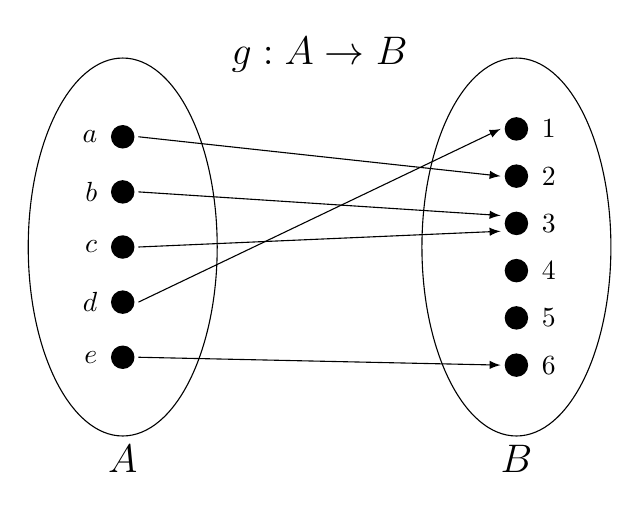
\begin{tikzpicture}[scale=1]
            \foreach \x in  {1,...,6}
            {
                \node at (5, -\x*0.6)[circle,fill,inner sep=3pt]{};
                \draw[shift={(5.2, -\x*0.6)}] node[right] {$\x$};
            }
            \draw (5,-2.1) ellipse (1.2 and 2.4);
    
            \foreach \x/\s in  {1/a,2/b,3/c,4/d,5/e}
            {
                \node at (0, -\x*0.7)[circle,fill,inner sep=3pt]{};
                \draw[shift={(-0.2, -\x*0.7)}] node[left] {$\s$};
            }
            \draw (0,-2.1) ellipse (1.2 and 2.4);
    
            \draw[-latex] (0.2,-0.7) -- (4.8,-1.2); 
            \draw[-latex] (0.2,-1.4) -- (4.8,-1.7); 
            \draw[-latex] (0.2,-2.1) -- (4.8,-1.9); 
            \draw[-latex] (0.2,-2.8) -- (4.8,-0.6); 
            \draw[-latex] (0.2,-3.5) -- (4.8,-3.6);
            
            \node[below] at (0, -4.5){\Large $A$};
            \node[below] at (5, -4.5){\Large $B$};
            \node[above] at (2.5, 0){\Large $g:A \to B$};
        \end{tikzpicture}}
    \end{center}

    定义 $Z_1 = \{1, 2, 3\}, Z_2 = \{2, 3, 4\}, Z_3 = \{4, 5, 6\}$。

    下面识别并解释以下原像:
    \begin{enumerate}[label=(\arabic*)]
        \item $\pim_g(\{1\}) = \{d\}$ \\
            因为 $g(d) = 1$,且不存在其他 $x \in A$ 满足 $g(x) = 1$。\\
            (注意,这里需要使用\emph{大括号}。``$\pim_g(1)$'' 是没有意义的。)
        \item $\pim_g(\{4\}) = \varnothing$ \\
            因为不存在 $x \in A$ 满足 $g(x) = 4$。
        \item $\pim_g(Z_1) = \{a, b, c, d\}$ \\
            因为 $g(a) = 2, g(b) = g(c) = 3, g(d) = 1$,且不存在其他 $x \in A$ 满足 $g(x) \in Z_1$。
        \item $\pim_g(Z_2) = \{a, b, c\}$ \\
            因为 $g(a) = 2, g(b) = g(c) = 3$,且不存在其他 $x \in A$ 满足 $g(x) \in Z_2$。
        \item $\pim_g(Z_3) = \{e\}$ \\
            因为 $g(e) = 6$,且不存在其他 $x \in A$ 满足 $g(x) \in Z_3$。
        \item $\pim_g(\{5\}) = \varnothing$ \\
            因为 $\forall x \in A \centerdot g(x) \ne 5$。
    \end{enumerate}
\end{example}

\begin{example}
    设函数 $f : \mathbb{R} \to \mathbb{R}$ 定义为 $\forall x \in \mathbb{R} \centerdot f(x) = x^2$。

    下面列出若干该函数的原像。请自行验证结论并尝试给出解释与证明。

    \begin{enumerate}[label=(\arabic*)]
        \item $\pim_f (\{1\}) = \{-1, 1\}$
        \item $\pim_f (\{y \in \mathbb{R} \mid y < 0\}) = \varnothing$
        \item $\pim_f (\{y \in \mathbb{R} \mid y \ge 0\}) = \mathbb{R}$
        \item $\pim_f (\{y \in \mathbb{R} \mid 0 < y < 1\}) = \{x \in \mathbb{R} \mid -1 < x < 1\}$
    \end{enumerate}
\end{example}